\documentclass[11pt,a4paper]{letter}
\usepackage[top=0.50in, bottom=0.5in, left=1.1in, right=1.1in]{geometry}
\usepackage{graphicx}

%\signature{}

\usepackage{Sweave}
\begin{document}

\begin{letter}{}

\includegraphics[width=0.3\textwidth]{logo_uah.png}

\opening{Dear Dr. Wake:}

\noindent Please consider our paper, entitled `Phylogenetic estimates of species-level phenology improve ecological forecasting' as an Article in \emph{Nature Climate Change}. Our research addresses the critical challenge of accurately predicting the impacts of climate change on plant phenology---with consequences for key ecosystem services---and highlights the importance of incorporating both species variability and phylogenetic information in forecasts.
\vspace{1.5ex}\\
Ecological forecasts often rely on unevenly sampled data across a limited number of species, resulting in predictions that fail to capture the high variability observed across species' responses. Recently, hierarchical mixed models have increased in popularity to address some of these issues, especially the common reality where some species are more data-abundant than others. Such models, however, violate our understanding of evolution by implicitly assuming all species are equally interchangeable. Instead, phylogeny highlights that species are nested within lineages and share a large, but variable, proportion of their evolutionary history with one another. % These models allow inference across species by pooling estimates of data-poor species towards those which are more data-rich.
\vspace{1.5ex}\\
Here, we propose a novel approach that uniquely incorporates shared evolutionary history into hierarchical models to inform species-level responses. We demonstrate how this new approach improves upon commonly used hierarchical mixed models by reducing forecasted uncertainty overall but increasing variation across species. For spring phenology we show that species-level variability is greater than variability across temperature and daylength cues, emphasizing the importance of accounting for species differences in ecological forecasting. This finding suggests the current focus on differences between phenological cues misses a much larger driver of variation. In addition, we show that our approach provides insights into how different clades have evolved in response to multiple interacting environmental cues.
\vspace{0.25ex}\\
Our results have important implications for improving ecological forecasting with continued climate change. As spring phenology impacts a suite of ecosystem services, including carbon sequestration, our new estimates can be scaled up to impact forecasts of climate change itself. At the same time our novel approach extends to forecasting far beyond the case study of phenology we present here.
\vspace{1.5ex}\\
We believe that our manuscript aligns well with the scope and objectives of \emph{Nature Climate Change}, and we have not submitted it elsewhere. We have suggested three possible reviewers (see online submission system: Carl Boettinger, Meredith Zettlemoyer, David Inouye). We are grateful for your consideration, and look forward to hearing from you.


\vspace{1.5ex}\\
\noindent Sincerely,\\
\vspace{1.5ex}\\
 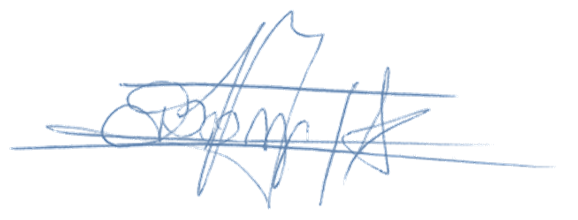
\includegraphics[width=0.2\textwidth]{Signature_IMC.png} \\
 \vspace{1.5ex}\\
\noindent Ignacio Morales-Castilla


\end{letter}
\end{document}
